\documentclass[12pt,openany,oneside]{report}
\usepackage[lined,algonl,boxed]{algorithm2e}
\usepackage{mathesis}
\usepackage{bm,graphicx,amsmath,amsfonts,makeidx,xcolor,hyperref}
\usepackage{mathrsfs,setspace}
\usepackage[small, bf]{caption}
\usepackage{chngcntr}
\counterwithout{footnote}{chapter}

\textheight 8.2in
\textwidth 5.5in
\topmargin -0.1in
\oddsidemargin 0.5in
\evensidemargin 0.5in

\renewcommand{\baselinestretch}{1.37}

\bibliographystyle{plain}

\makeindex

\begin{document}

\def\thechapter       {\arabic{chapter}}
%\def\thesection       {\arabic{chapter}.\Alph{section}}
\def\thefigure        {\arabic{chapter}.\arabic{figure}}
\def\theequation      {\arabic{chapter}.\arabic{equation}}

% uncomment this line when submitting to Library and Archives Canada,
% as they need a single-sided version.
\setboolean{@twoside}{true}

\flushbottom
\thispagestyle{empty}

%\begin{asydef}
%// Global definitions can be put here.
%\end{asydef}


%%%%%%%%%%%%%%%%%%%%%%%%%%%%%%%%%%%%%%%%%%%%%%%%%%%%%%%%%%%%%%%%%%%
%%%%%%%%%%%%%%%%%%%%%%%%%%%%%%%%%%%%%%%%%%%%%%%%%%%%%%%%%%%%%%%%%%%
%%%%%%%%%%%%%%%%%%%%%%%%%%%%%%%%%%%%%%%%%%%%%%%%%%%%%%%%%%%%%%%%%%%
% this sets the metadata for the PDF (if compiled with pdflatex)
% FILL THIS IN!!!
\def\ThesisTitle{The Title of the Thesis}
\def\ThesisAuthor{Author's Name}
% convocation date must either be ``Spring 20xx'' or ``Fall 20xx''
\convocationdate{Spring 2012}
\degree{Doctor of Philosophy}
%\degree{Masters of Science}

\supervisor{Dr.\ Supervisor}
%\cosupervisor{your co-supervisor} % if applicable
\firstcommitteemember{Dr.\ Committee Person}
\secondcommitteemember{Dr.\ Committee Person}
%\thirdcommitteemember{}
%\fourthcommitteemember{}
%\fifthcommitteemember{}

\department{Department of Mathematical and Statistical Sciences}
% If you have a specialization, enter it here
\fieldofstudy{Mathematics}
%%%%%%%%%%%%%%%%%%%%%%%%%%%%%%%%%%%%%%%%%%%%%%%%%%%%%%%%%%%%%%%%%%%
%%%%%%%%%%%%%%%%%%%%%%%%%%%%%%%%%%%%%%%%%%%%%%%%%%%%%%%%%%%%%%%%%%%
%%%%%%%%%%%%%%%%%%%%%%%%%%%%%%%%%%%%%%%%%%%%%%%%%%%%%%%%%%%%%%%%%%%


\definecolor{heavyblue}{cmyk}{1,1,0,0.25}
\hypersetup{
  pdftitle=\ThesisTitle,
  pdfauthor=\ThesisAuthor,
  pdfpagemode=UseOutlines,
  citebordercolor=0 0 1,
  colorlinks=true,
  allcolors=heavyblue,
  breaklinks=true,
  pdfpagetransition=Dissolve,
  bookmarks=true
}
\title{\ThesisTitle}
\author{\ThesisAuthor}

\beforebodyoftex

\titlepage

\newpage\setcounter{page}{0}\thispagestyle{empty}$\text{ }$
\newpage\setcounter{page}{2}

%\libraryreleaseform %%% not currently required by FGSR
%\signaturepage %%% not currently required by FGSR

%\begin{dedication}
% put your dedication here
%\end{dedication}

\doublespacing

\newpage
\begin{abstract}
  Witty and concise abstract.  References to \cite{MathStats38} and
  \cite{Physicist38}.
\end{abstract}

% 1.5 line spacing is allowed after the abstract
\onehalfspacing

%\begin{preface}
% preface? we don't need no stinking preface.
%\end{preface}

\begin{acknowledgement}
  Heartfelt acknowledgements.
\end{acknowledgement}



\tableofcontents

% if you have no tables, please comment-out this line:
\listoftables

% if you have no figures, please comment-out this line:
\listoffigures

% list of symbols is optional here. use f.ex. longtable package:
%\chapter*{List of Symbols}

\beginbodyoftex

%%%%%%%%%%%%%%%%%%%%%%%%%%%%%%%%%%%%%%%%%%%%%%%%%%%%%%%%%%%
%%%%%%%%%%%%%%%%%%%%%%%%%%%%%%%%%%%%%%%%%%%%%%%%%%%%%%%%%%%
%%%%%%%%%%%%%%%%%%%%%%%%%%%%%%%%%%%%%%%%%%%%%%%%%%%%%%%%%%%


\chapter{Introduction}

Introduction!

Also, Table~\ref{egtable}.

\begin{table}[htbp]
  \begin{center}
    \begin{tabular}{|p{4cm}|p{4cm}|}
      \hline
      Spring 20xx & Fall 20xx \\
      \hline
      \hline
      if submitting between Oct 1--April 15
      & if submitting between April 16--Sept 30\\
      \hline
    \end{tabular}
    \caption{Convocation date}
    \label{egtable}
  \end{center}
\end{table}


\chapter{Super-Cool Stuff}

It really is pretty cool.  Consider the Venn diagram in Figure~\ref{venn}.

\begin{figure}[htbp]
  \begin{center}
    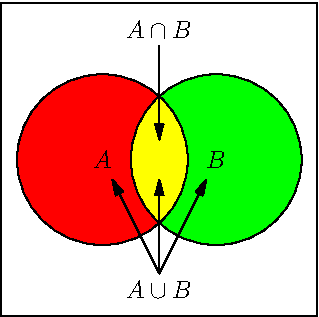
\includegraphics{venn}
    \caption{A Venn diagram}
    \label{venn}
  \end{center}
\end{figure}



\chapter{Conclusion}

We should really get a beer now.

\singlespacing
{
\bibliography{refs}
}

\vfill
\textheight 9in
\eject
\topmargin -1in
\clearpage
\phantomsection
\addcontentsline{toc}{chapter}{Index}
\printindex

\end{document}
